\subsection{Insights from Experimental Observations}


% ---------------- Figure ----------------
\begin{figure*}[t]               % use figure instead of figure* for 1‑column
  \centering
  % ---------- first row ----------
  \subcaptionbox{MMLU-Llama3.2\label{fig:plotA}}[0.30\textwidth]{%
    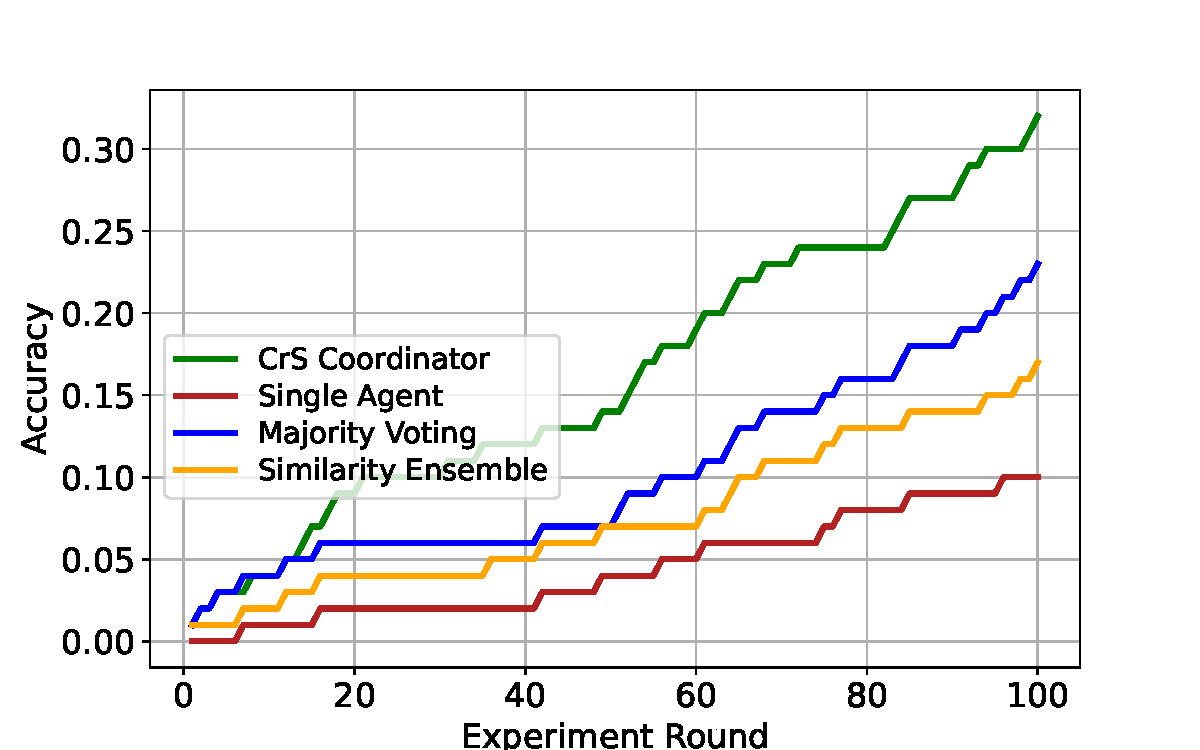
\includegraphics[width=\linewidth]{plots/baselines_llama3.2_mmlu.pdf}}
  \hfill
  \subcaptionbox{MMLU-Mistral\label{fig:plotB}}[0.30\textwidth]{%
    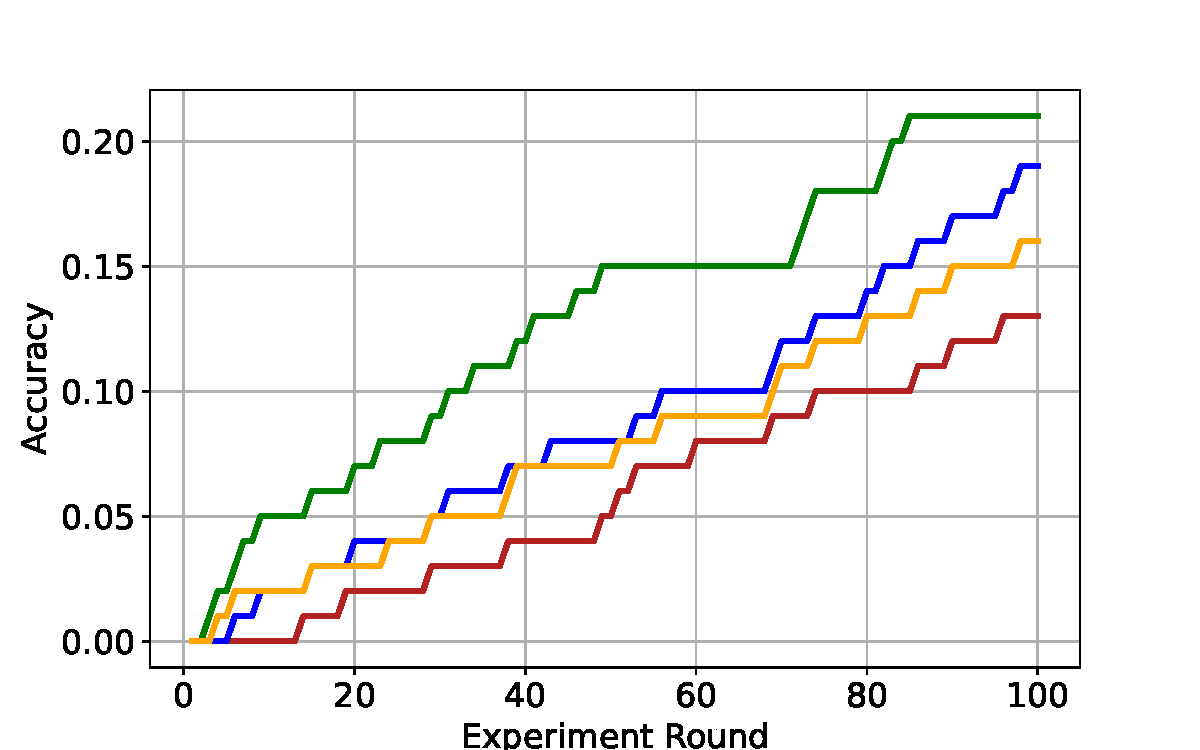
\includegraphics[width=\linewidth]{plots/baselines_mistral7b_mmlu.pdf}}
  \hfill
  \subcaptionbox{MMLU-Qwen2.5\label{fig:plotC}}[0.30\textwidth]{%
    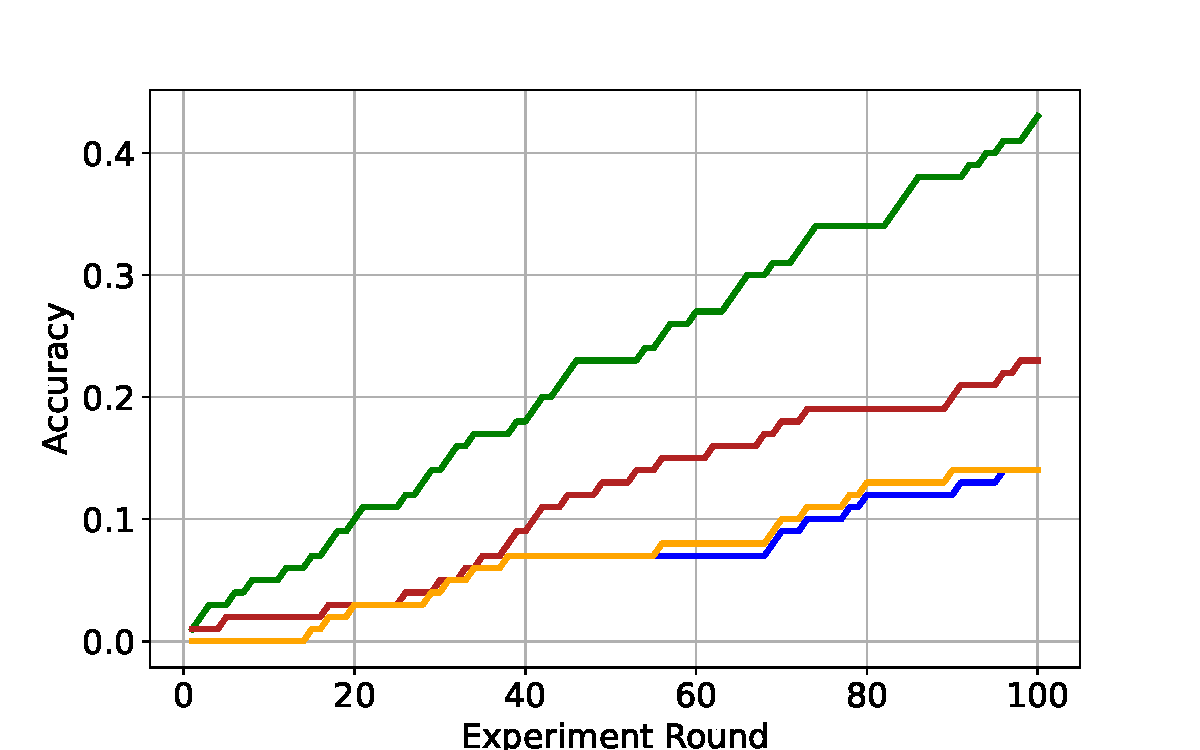
\includegraphics[width=\linewidth]{plots/baselines_qwen2.5_mmlu.pdf}}

  % \vspace{0.8em} % small vertical gap between rows
  \vspace{-1mm}

  % ---------- second row ----------
  \subcaptionbox{GSM8K-Llama3.2\label{fig:plotD}}[0.30\textwidth]{%
    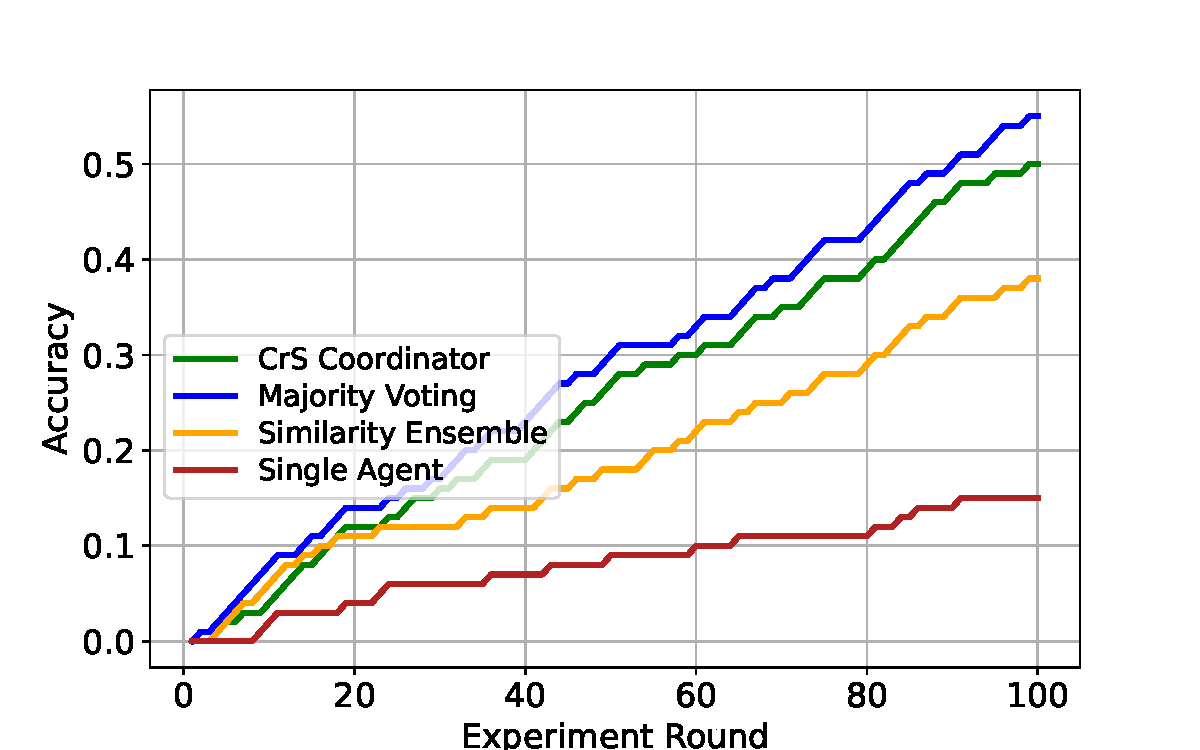
\includegraphics[width=\linewidth]{plots/gms8k_baselines_llama3.2-2.pdf}}
  \hfill
  \subcaptionbox{GSM8K-Mistral\label{fig:plotE}}[0.30\textwidth]{%
    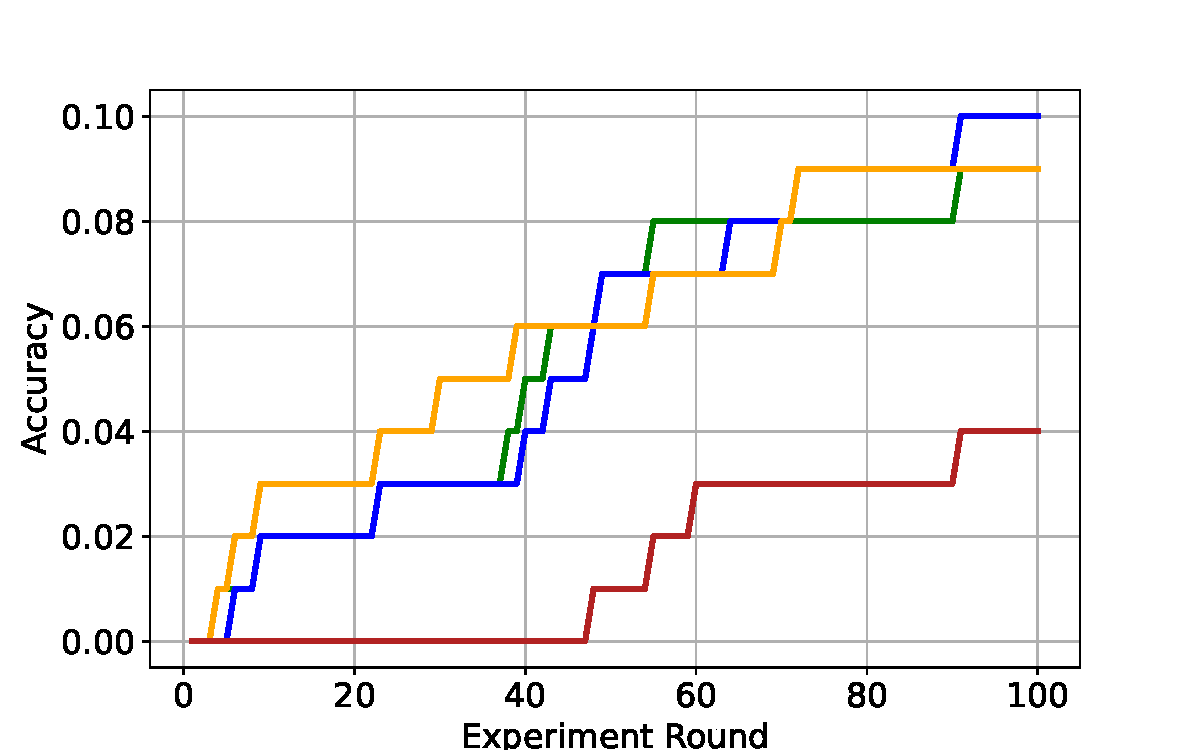
\includegraphics[width=\linewidth]{plots/gms8k_baselines_mistral7b-2.pdf}}
  \hfill
  \subcaptionbox{GSM8K-Qwen2.5\label{fig:plotF}}[0.30\textwidth]{%
    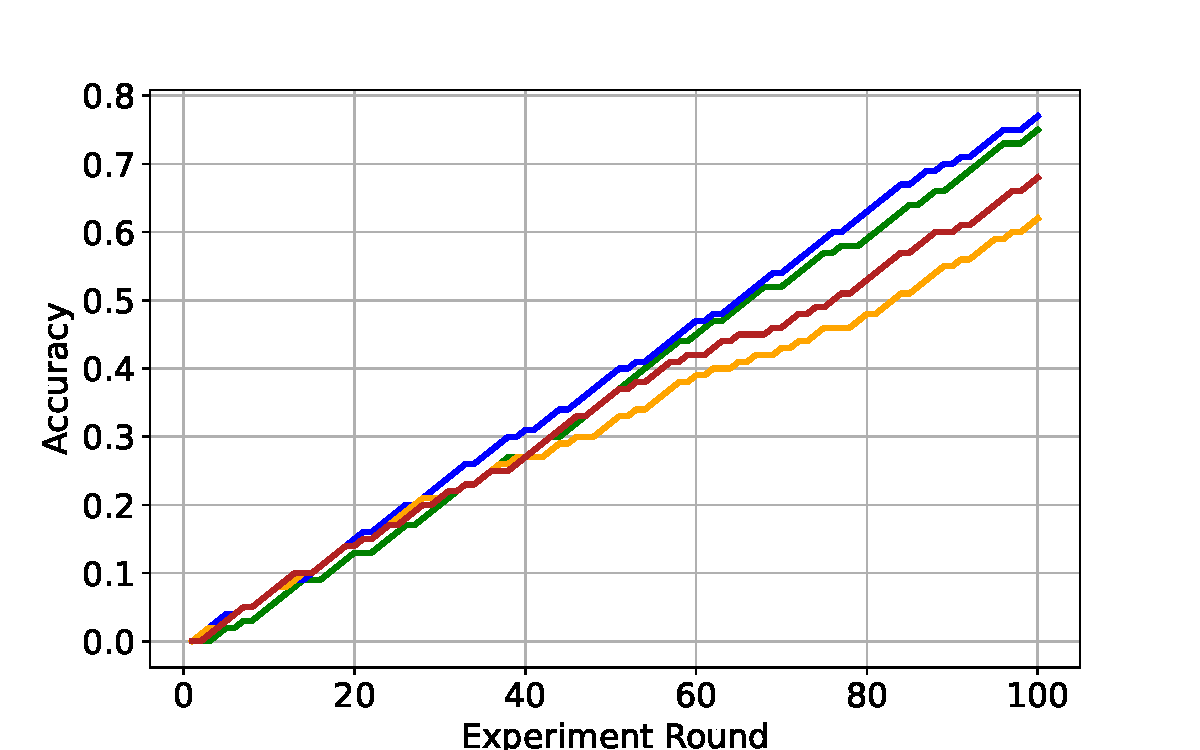
\includegraphics[width=\linewidth]{plots/gms8k_baselines_qwen2.5-2.pdf}}

  \caption{Performance comparison of baseline methods versus CrS‑based coordinators.}
  % with the CrS results split to highlight differences between mathematical‑reasoning tasks (GSM8K) and multiple‑choice question answering (MMLU-MS).
  \label{fig:sixplots}
  \vspace{-2mm}
\end{figure*}


 \begin{figure}[ht]
    \centering
    \begin{minipage}[b]{0.8\columnwidth}
    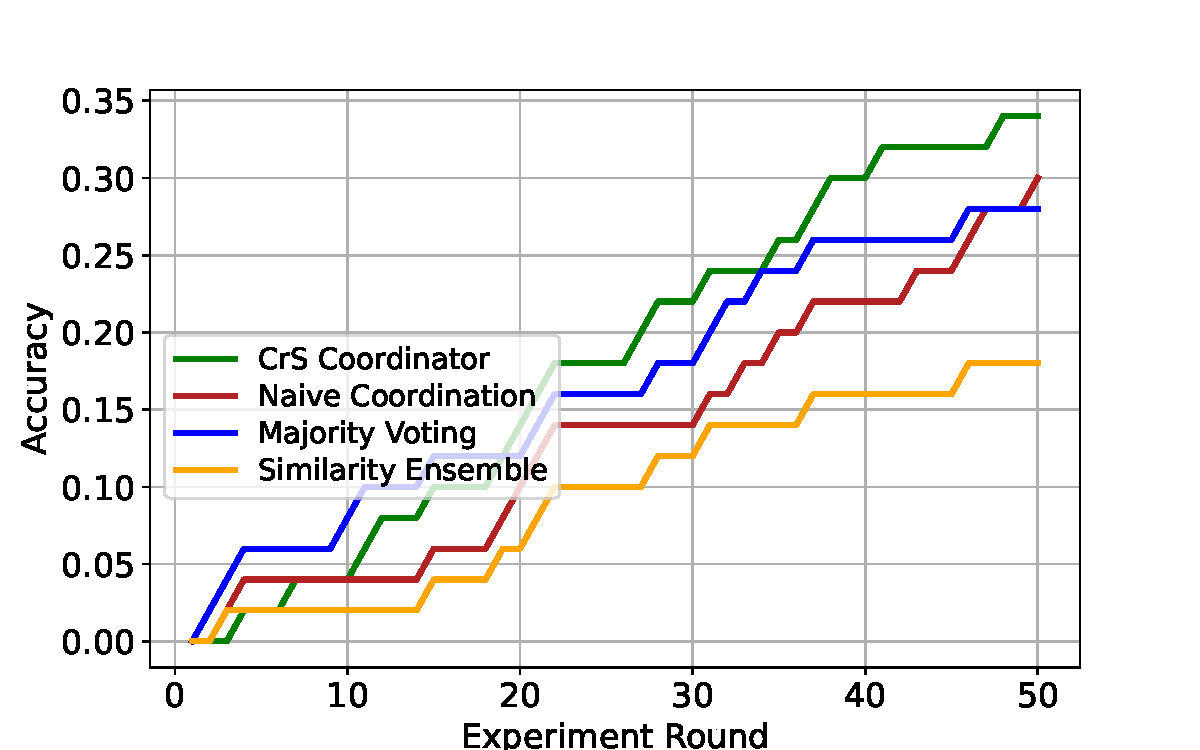
\includegraphics[width=\textwidth]{plots/chain_baseline_mmlu_4adv.pdf}
    \caption{Baseline accuracy for a five‑agent chain (one faithful, four adversarial). The “CrS Coordinator” (green) curve reflects a CrS‑ordered chain, whereas all other methods use an unordered chain topology.}
    \label{fig:chain-baseline}
    \end{minipage}
    \vspace{-3mm}
\end{figure}



\subsubsection{Credibility Scores Drive Consistent Gains}
Across \textbf{all four benchmarks} (MMLU, GSM8K, MATH, ResearchQA) and for \textbf{every backbone} (LLaMA3.2, Mistral7B, Qwen2.57B), introducing our Credibility Score (CrS) raises accuracy by \emph{6--30 percentage points}. In high--noise settings such as GSM8K with three adversaries, CrS lifts LLaMA3.2 from \textbf{23\%$\rightarrow$42\%} in CrS-ordered chain and Qwen2.5 from \textbf{65\%$\rightarrow$75.5\%} in SIA. These patterns confirm that weighting agent opinions by empirically-measured reliability is a general mechanism for mitigating adversarial influence. 

Table~\ref{tab:SAA} presents results for Standalone Agent Architecture (SAA), which features no inter-agent interactions and utilizes a centroid-based aggregator inspired by~\cite{requal} as the coordinator. Our findings reveal consistent improvements in the number of correct responses. Specifically, in mathematical reasoning tasks such as GSM8K and MATH, the use of CrS coordination enhances the rate of fully correct responses $(r=1.0)$. This improvement occurs primarily by reducing the partially correct responses $(0.5 \leq r < 1.0)$, achieved through assigning higher weights to answers from more credible agents.
% \mohsen{Did we discuss anywhere what 'partially correct response' means?} \sana{No but it's basically means $(0.5 \leq r < 1.0)$ which I metioned. MMLU-MS does not have that because it's a multi-choice question answering which is either correct or not which means (r=1.0 or -1.0)}

\subsubsection{Reasoning vs Multi-Choice Tasks}
% \vspace{-1mm}
We implement all three baseline models on an identical topology, utilizing the same agents to ensure consistency. Thus, the sole differentiating factor across these baselines is the coordination mechanism, allowing for a fair and precise comparison among models. Figure~\ref{fig:plotA},~\ref{fig:plotB} and ~\ref{fig:plotC}  illustrates that across 100 evaluated questions, the CrS coordinator consistently outperforms other baseline methods when confronted with a majority of adversarial agents. Interestingly, Majority Voting emerges as the second most effective coordination method after CrS. This result may initially seem counterintuitive, given that a majority of agents are adversarial and therefore expected to provide incorrect responses. However, as demonstrated in Table~\ref{tab:example-table-1}, adversaries occasionally alter their initial responses, eventually aligning with the correct solution. This phenomenon can be explained in two ways: 1) adversaries sometimes strategically shift their responses after misleading other agents to avoid revealing their adversarial nature; and 2) \textbf{adversaries can be influenced and persuaded by faithful agents}, prompting them to correct their earlier mistakes. Consequently, if at least one faithful agent consistently maintains the correct response, Majority Voting can yield accurate outcomes in specific scenarios. Nonetheless, these occasional successes are insufficient to prevent an overall decline in accuracy, reinforcing the superior robustness of the CrS coordinator against adversarial influence on MMLU-MS.
Figures~\ref{fig:plotD}, \ref{fig:plotE}, and \ref{fig:plotF} illustrate the performance of CrS on mathematical reasoning tasks using the GSM8K dataset. In these experiments, CrS achieves the second-best results, trailing behind Majority Voting. We attribute this performance gap to the intricate process of calculating Contribution Scores (CSc) in mathematical reasoning, where the complexity of reasoning significantly increases the likelihood of errors. These inaccuracies can corrupt the credibility score calculations and weighting mechanisms used by the CrS coordinator, occasionally resulting in the inadvertent prioritization of adversarial responses. This issue does not arise in Majority Voting. Nevertheless, despite these challenges, the CrS coordinator consistently outperforms Single Agent, Similarity Ensemble and naive coordination(Table~\ref{tab:progress-results}).
   

\begin{table}[t]            % stays in one column
  % \centering
  \small                    % 
  \caption{Standalone Agent Architecture with LLaMA3.2(3B) agents. The table shows coordinator accuracy using credibility‑score (CrS) weights versus uniform weights across all tasks; numbers in parentheses indicate the resulting performance gap.}
  \label{tab:SAA}
  \begin{tabularx}{\columnwidth}{l|CC}  % four centred columns
    \hline
    \textbf{Dataset} & \textbf{\parbox[c]{2cm}{\raggedright Correct\\$(r=1.0)$}} & \textbf{\parbox[c]{2cm}{\raggedright Partially \\Correct$(0.5\le r<1.0)$}}  \\ \hline
    GSM8K & 57.6(\textcolor{darkgreen}{$+3.6\%$}) & 9.9(\textcolor{red}{$-1.6\%$}) \\
    MATH & 32.75(\textcolor{darkgreen}{$+5.75\%$}) & 13.3(\textcolor{red}{$-5.7\%$}) \\
    ResearchQA & 0.0 & 89.0(\textcolor{darkgreen}{$+2\%$}) \\
    MMLU-MS & 37.0(\textcolor{darkgreen}{$+2\%$})& - \\ \hline
  \end{tabularx}
  \vspace{-4mm}
\end{table}
\vspace{-1mm}
\subsubsection{Model Capacity Matters But Only With Coordination}
Small models (e.g., Mistral7B on MATH) suffer the steepest drops when exposed to adversaries: their multi-agent accuracy falls by up to \textbf{50\%} ($6/12$, Table~\ref{tab:progress-results}). CrS partially restores performance (\textasciitilde6pp gain), yet never reaches the ceiling attained by larger or instruction-tuned models. This suggests that \emph{coordination cannot fully compensate for insufficient backbone reasoning capacity}; future work might explore knowledge-distillation style training to narrow this gap.

\subsubsection{Judge-Computed CrS Imitates the Shapley Value }
\label{sec:exp:judge}

We illustrate the progression of CrS in Figures~\ref{fig:judge-weight} and \ref{Crs-Shapley}. Specifically, Figure~\ref{fig:judge-weight} presents the CrS evolution for Qwen2.5 agents on GSM8K—achieving the highest overall accuracy—and LLaMA3.2 agents on ResearchQA—demonstrating the greatest accuracy improvements, as detailed in Table~\ref{tab:progress-results}. The calculated CrS values effectively reflect agent credibility by appropriately down-weighting adversarial agents based on their contribution and reward metrics. Importantly, these CrS values closely approximate the Shapley value-based CrS used in the Standalone Agent Architecture (SAA), as evidenced by the consistent patterns in CrS progression and empirical outcomes. Further comparative results for both SAA and Stochastic Interaction Architecture (SIA) involving two agents (including one adversarial agent) are presented in Figures~\ref{crs-saa} and \ref{crs-sia} in Appendix~\ref{app:exp-ext}.
% \subsection{Communication History as an Implicit Memory}
% Reusing the \emph{same} coordinator following the CrS-driven pre-processing phase within the stochastic architecture and constructing the chain architecture without sorting agents by their credibility scores results in accuracy improvements ranging from 2\% to 16\%, compared to initiating a fresh coordinator. We hypothesize that the coordinator implicitly learns soft heuristics about each agent's writing style and typical error patterns—effectively an implicit memory absent in new coordinator instances.

% This intuition is further tested through a targeted ablation study described in Section~\ref{sec:ablation}.

\subsubsection{Judge Alters the Outcome}

\begin{table}[h!]
\centering
\resizebox{0.9\columnwidth}{!}{%
\begin{tabular}{@{}lc|cc@{}}
\toprule
 & Pre-Communication & \multicolumn{2}{c}{Post-Communication} \\ 
&   & Chain & Random \\ 
\midrule
\textbf{CrS Coord.} & - & $0.16$& $0.12$ \\ 
Single Agent-LLaMa3.2(3B) & $0.32$ & $0.16$ & $0.16$\\ 
\bottomrule
\end{tabular}%
}

% Llama 3.2        & $0.01$  & $0.14$&$0.10$ \\ 
\caption{Comparison of accuracies before and after communication on a sample of 50 questions from HumanEval dataset.}
\label{tab:humaneval_comp}
\vspace{-2mm}
\end{table}

Replacing GPT-4o mini with a less capable judge, such as LLaMa3.2 (3B), leads to significant declines in accuracy—even when employing CrS—as erroneous evaluations of contribution scores (CSc) corrupt the credibility metrics essential for updating agent credibility. For instance, Qwen2.5 achieves the highest accuracy on GSM8K, as indicated in Table~\ref{tab:progress-results}, but using Llama3.2 (3B) as the evaluator decreases this accuracy by 54\%. This clearly demonstrates the critical dependence of CrS effectiveness on the evaluator's quality. A comparison between Figure~\ref{fig:llama-judge} in Appendix~\ref{app:exp-ext} and Figure~\ref{fig:judge-weight} further supports this conclusion.

Another issue arises when the judge is not capable of accurately evaluating the final response and providing a correct reward signal ($r$). This problem was particularly noticeable in our experiments on the HumanEval code completion benchmark using the GPT-4o mini judge (Table~\ref{tab:humaneval_comp}). These inaccurate evaluations, and the resulting miscalculations of Contribution Scores (CSc), significantly distort the Credibility Score (CrS) updates, ultimately undermining the overall effectiveness of the framework. While employing a more specialized and capable judge could reduce such inaccuracies, it also raises concerns about the practicality and necessity of the multi-agent configuration itself since directly assigning the task to a stronger evaluator might be more effective \footnote{A detailed analysis of the HumanEval results is provided in Appendix~\ref{app:exp-details}.}.

\subsubsection{Topology and Link Density}
% Structured (chain) communication amplifies the benefit of CrS for reasoning-heavy tasks such as ResearchQA (+20pp over stochastic), but harms performance on arithmetic-style MATH where early errors propagate linearly. 
\vspace{-2mm}
\begin{figure}[ht]
    \vspace{-2mm}
    \centering
    \begin{minipage}[b]{0.8\columnwidth}
    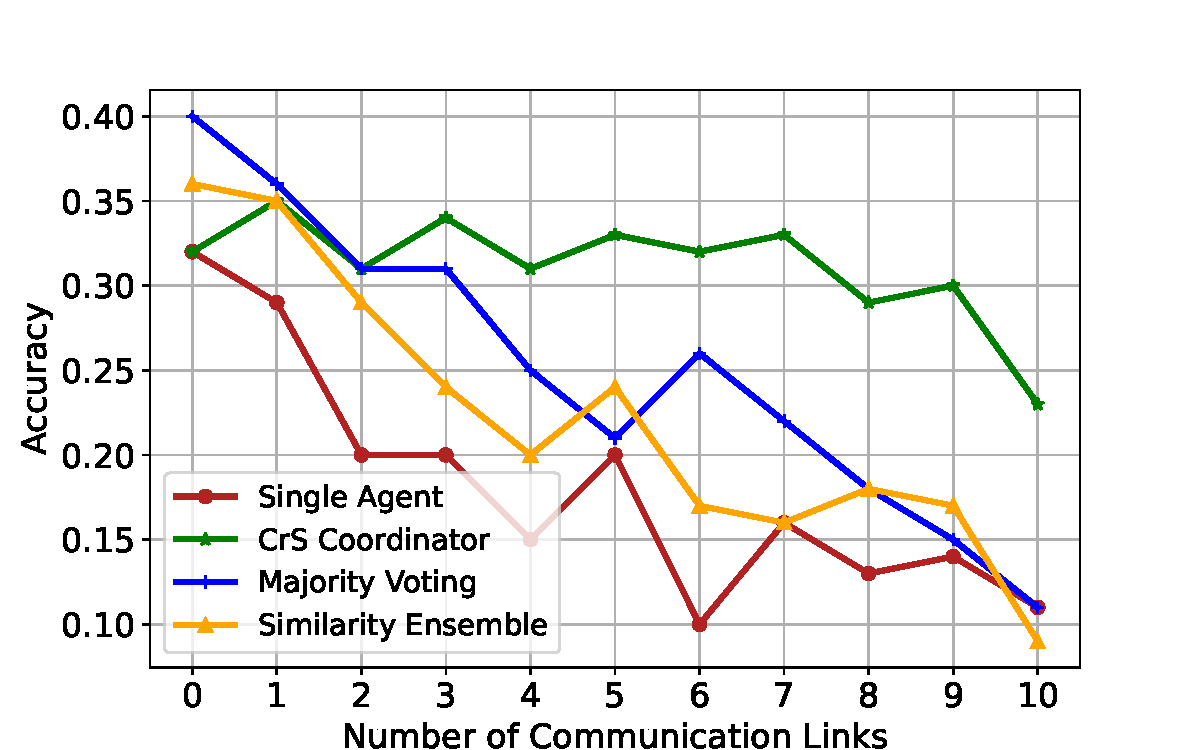
\includegraphics[width=\textwidth]{plots/number_of_links.pdf}  % adjust width here
    \caption{Impact of the number of communication links on accuracy across baseline methods compared to the CrS coordination mechanism on MMLU-MS. }
    \label{fig:n_link}
    \end{minipage}
    \vspace{-2mm}
\end{figure}
Figure~\ref{fig:n_link} demonstrates that increasing the communication link count in SIA beyond six edges results in diminishing returns. Specifically, accuracy saturates at six links and notably \emph{decreases} when exceeding seven links, likely due to information overload. Conversely, increasing the link count extends the length of the communication history shared with the judge for computing the Contribution Score (CSc). This extension raises two primary concerns:
1) Activation of the token compressor becomes necessary to reduce token count to adhere to the judge's token limit requirements. This will increase the runtime.
2) If one round of token summarization is insufficient to meet these token requirements, subsequent rounds of compression may be triggered. Multiple rounds of compression risk losing information deemed non-essential by the compressor, ultimately affecting the accuracy and reliability of the contribution score.

Our empirical results indicate that a configuration with six links represents the optimal balance, effectively facilitating the study of adversarial impacts while minimizing the frequency of triggering more than one compression cycle. Figure~\ref{fig:n_link} also highlights the stability of the CrS coordinator with increased intra-group communication compared to other baseline methods, which exhibit a sharp decline in accuracy and significant negative impacts from additional communication rounds. The CrS coordinator's performance surpasses other aggregation methods by approximately 10 percentage points.
\vspace{-2mm}
\subsubsection{Adversary Proportion}\label{sec:exp-adversary}
\vspace{-1mm}
\begin{figure}[ht]
    \vspace{-4mm}
    \centering
    \begin{minipage}[b]{0.8\columnwidth}
    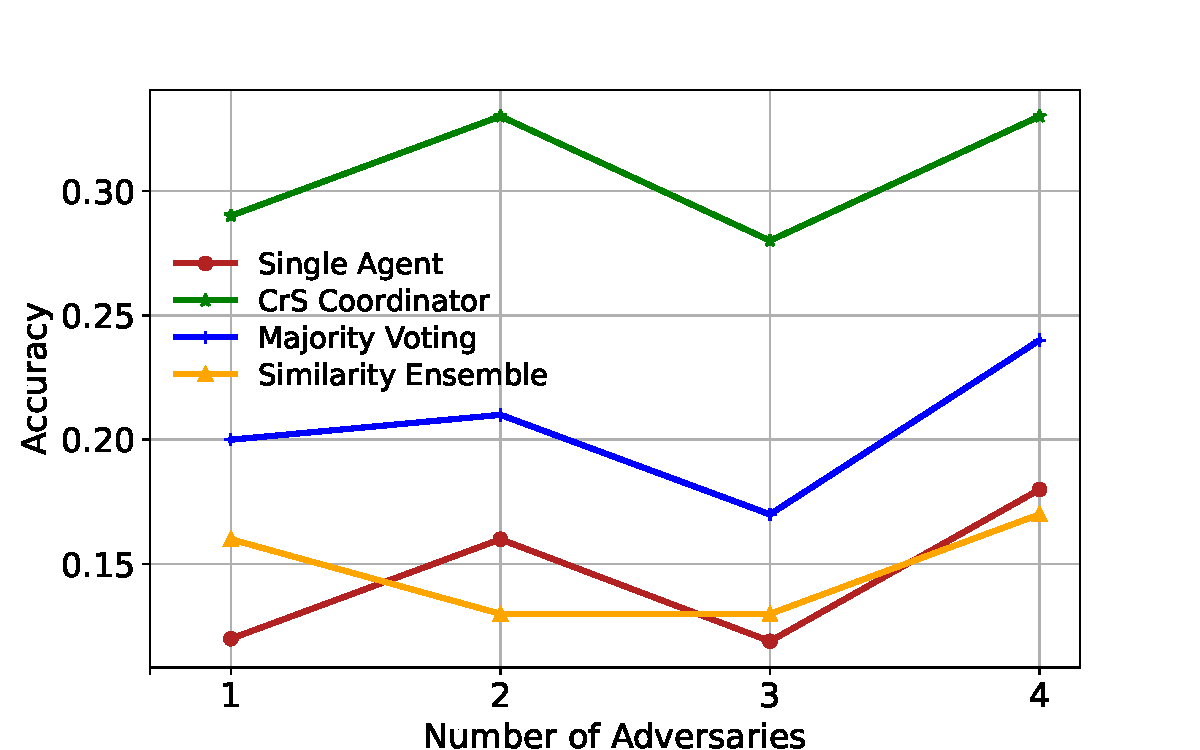
\includegraphics[width=\textwidth]{plots/number_of_adv.pdf}  % adjust width here
    \caption{Impact of adversarial agent count on accuracy across baseline methods compared to the CrS coordination mechanism on MMLU-MS.}
    \label{fig:n_adv}
    \end{minipage}
    \vspace{-3mm}
\end{figure}

Figure~\ref{fig:n_adv} demonstrates performance stability when employing CrS weighting: even with one to four adversaries present, accuracy consistently stays within a narrow range around 31\% ($\pm 2$ percentage points). In contrast, naive strategies experience significant fluctuations and never surpass 24\%. This stability indicates that reliability-based agent weighting effectively reduces sensitivity to adversary count, a promising outcome for scalability to larger and potentially noisier teams.

Figure~\ref{fig:chain-baseline} further supports this conclusion by demonstrating the superior performance of the CrS coordinator within a chain architecture, even under extreme adversarial conditions where 4 out of 5 agents are adversaries. These results validate our earlier findings in the Stochastic Interaction Architecture and suggest that the advantages of the CrS coordination mechanism extend reliably to structured communication topologies as well.

% \subsection{Insights}
% \begin{itemize}
% \item \textbf{Credibility signals are essential}: they convert noisy collective intelligence into robust gains.
% \item \textbf{Evaluator quality is a hidden bottleneck}: better judges beget better CrS and higher final accuracy.
% \end{itemize}

% \section{Ablation Study}\label{sec:ablation}
